%!TEX root = ../hbrs-poster.tex
\documentclass[hbrs-poster.tex]{subfiles}
\begin{document}
    \block{ Methodology}
    {
        In preprocessing step, we performed tokenization to convert text into tokens (words, sub-words, or characters) that the model can understand. Next steps included removing unnecessary characters, punctuation, or special symbols, normalization and lower casing, stemming and lemmatization.
                
        Next, we performed vectorization to encode text data into numerical format to capture the contextual features of the plot summaries and make them suitable for machine learning models. We utilized TF-IDF with ngram size (1,3) to capture more relationships between words. Finally, we trained our own language model as well as distinct classifiers and compared their results.
        \begin{tikzfigure} 
            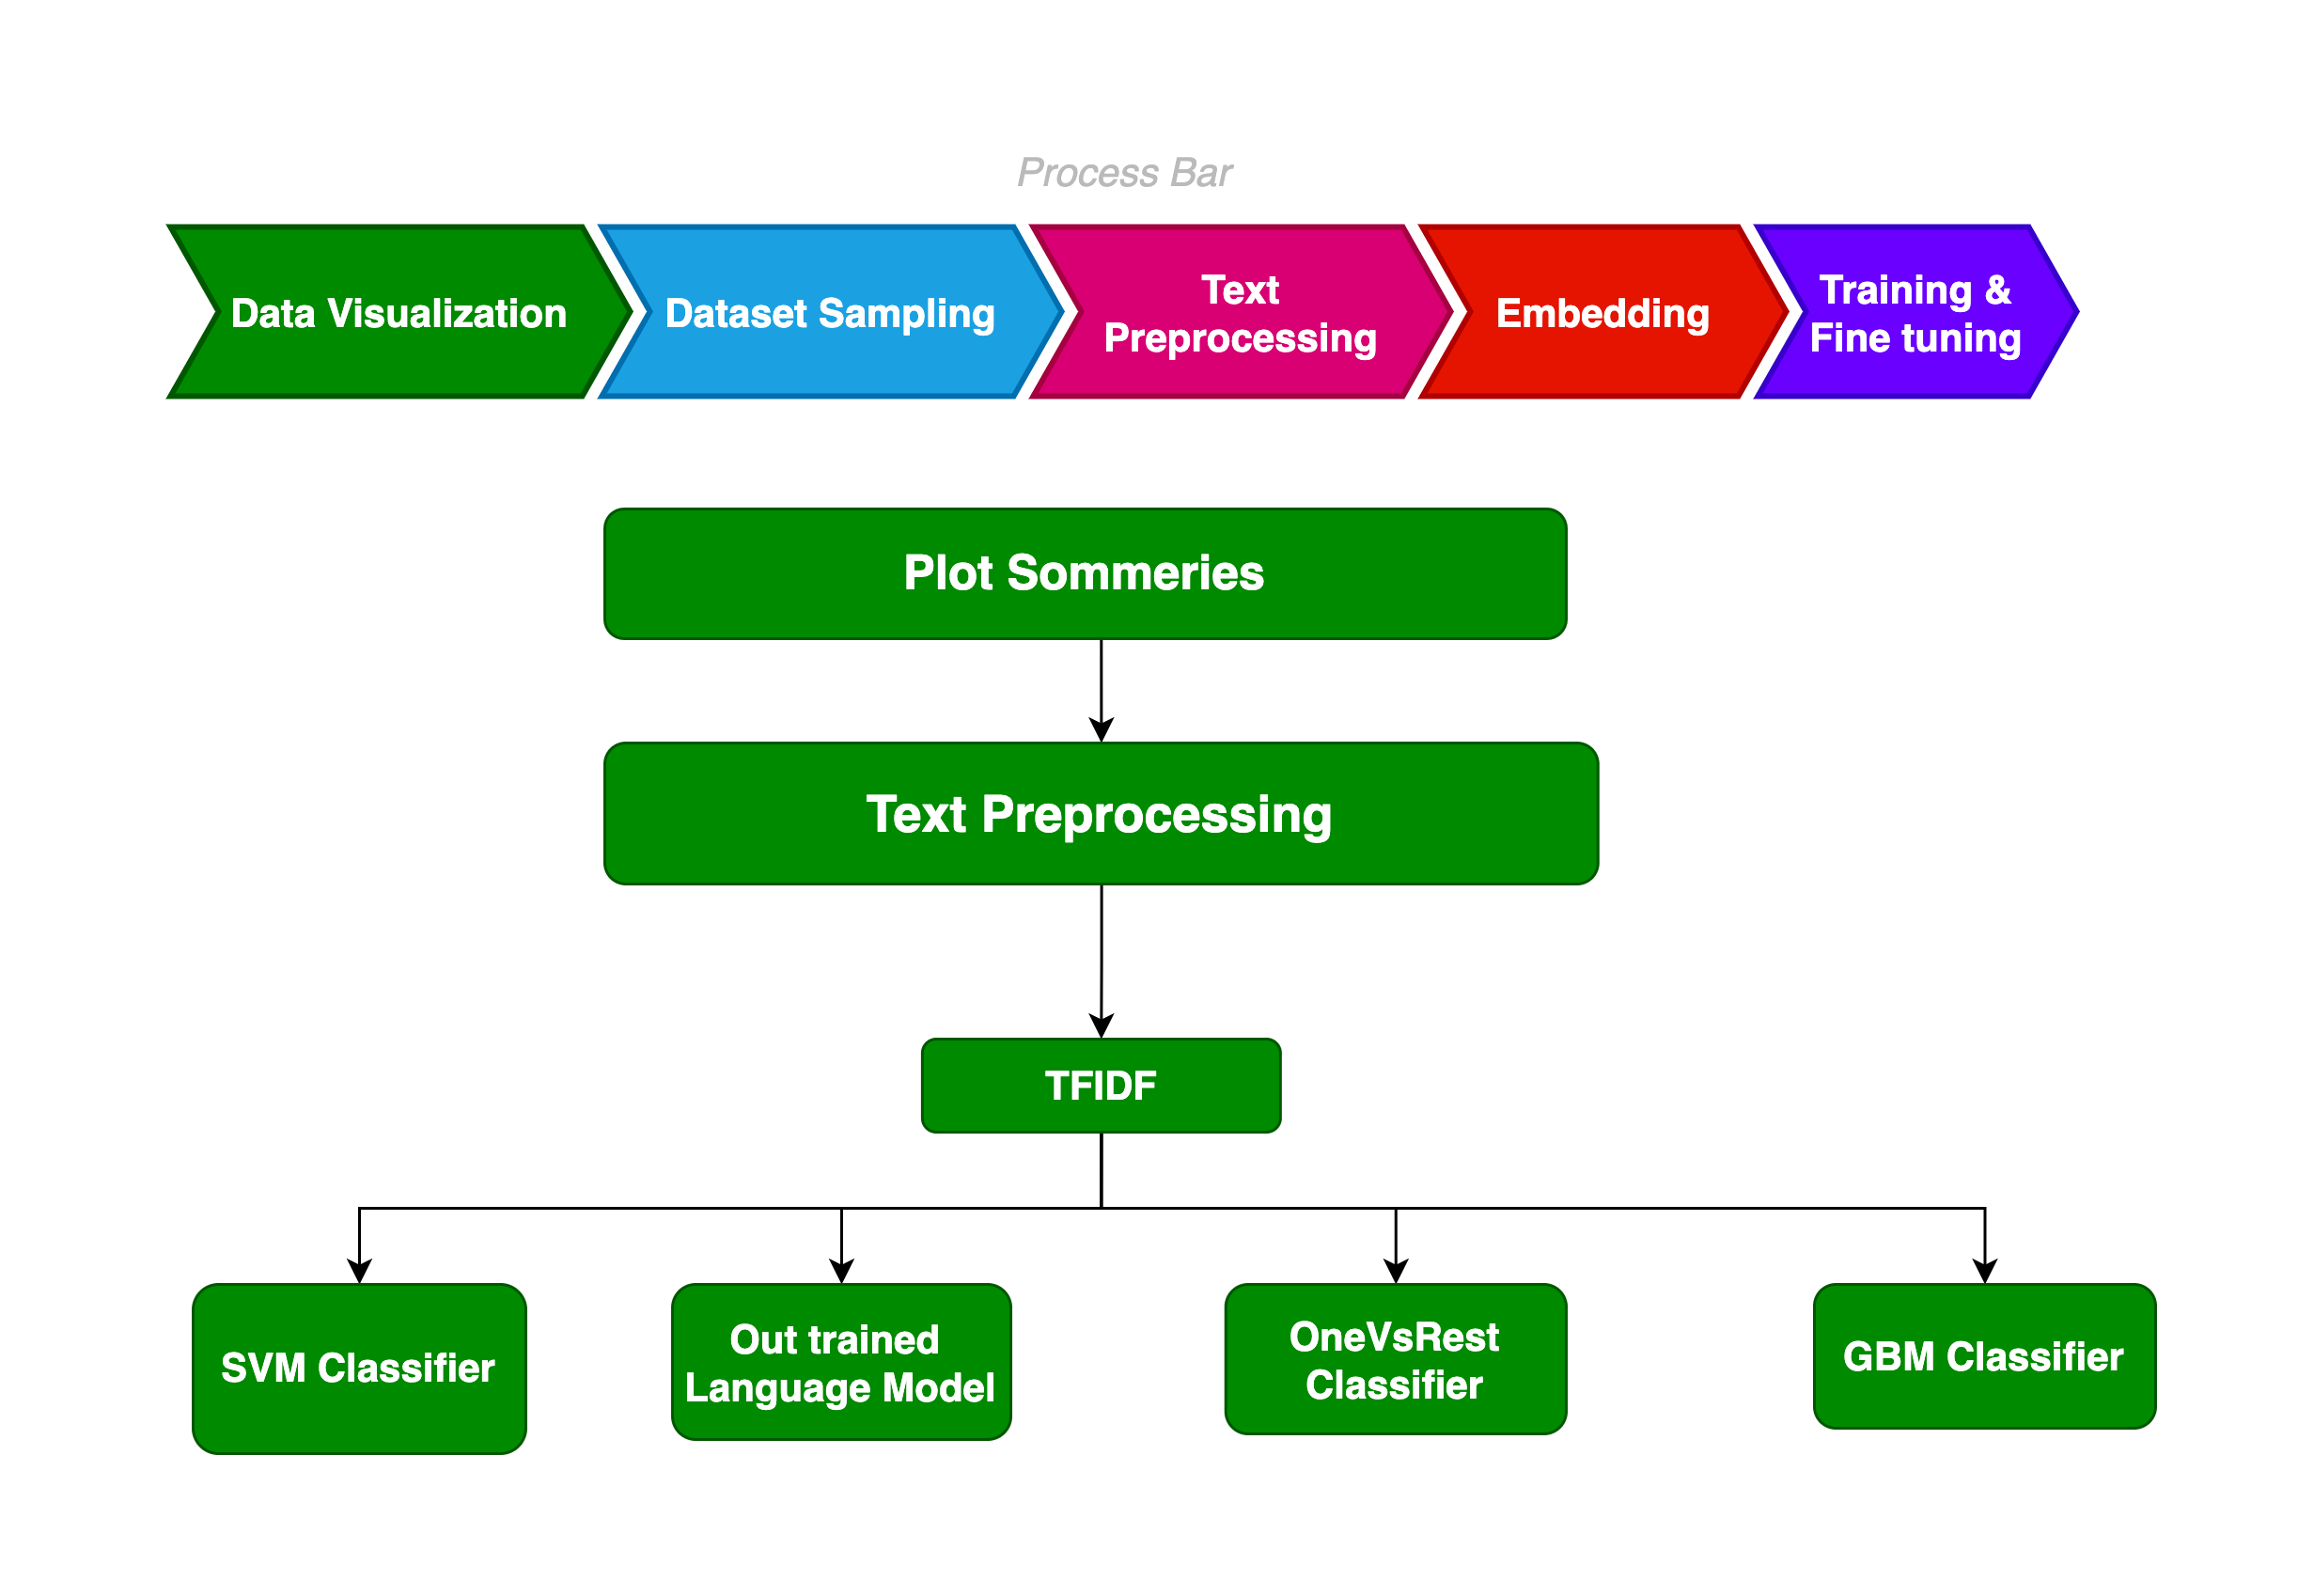
\includegraphics[width=0.43\textwidth, height=0.245\textheight]{figures/Unbenanntes Diagramm.png}
        \end{tikzfigure}

        \begin{tikzfigure}
            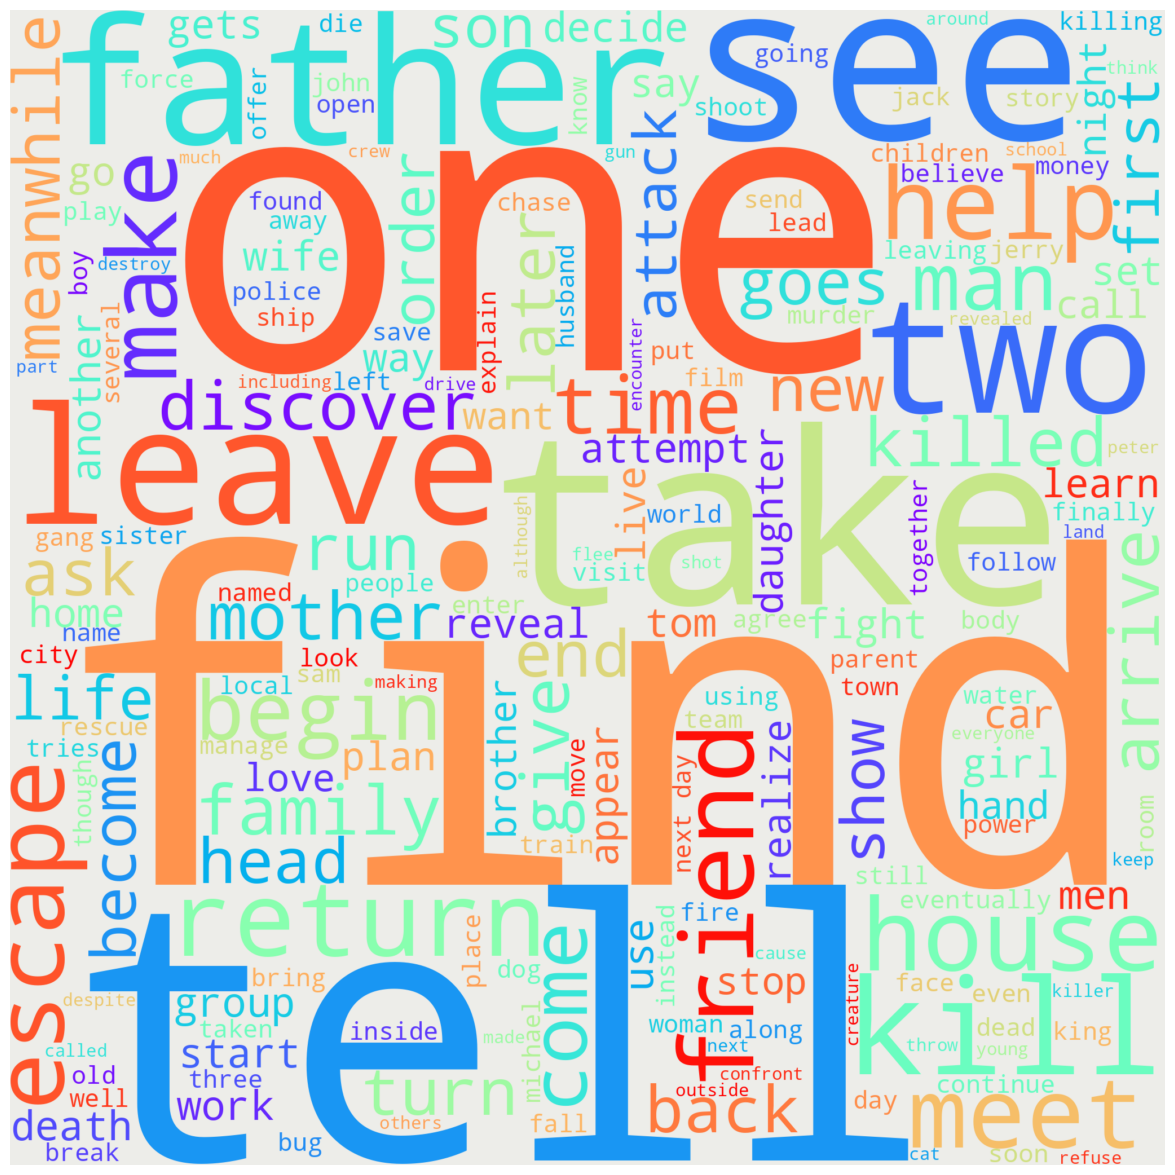
\includegraphics[width=0.35\textwidth, height=0.195\textheight]{figures/output4.png}
        \end{tikzfigure}
    }
\end{document}
